% Copyright (C) 2012 Shi.Zhan <g.shizhan.g@gmail.com>
%
% Permission is hereby granted, free of charge, to any person obtaining a copy of this software and associated documentation files (the "Software"), to deal in the Software without restriction, including without limitation the rights to use, copy, modify, merge, publish, distribute, sublicense, and/or sell copies of the Software, and to permit persons to whom the Software is furnished to do so, subject to the following conditions:
%
% The above copyright notice and this permission notice shall be included in all copies or substantial portions of the Software.
%
% THE SOFTWARE IS PROVIDED "AS IS", WITHOUT WARRANTY OF ANY KIND, EXPRESS OR IMPLIED, INCLUDING BUT NOT LIMITED TO THE WARRANTIES OF MERCHANTABILITY, FITNESS FOR A PARTICULAR PURPOSE AND NONINFRINGEMENT. IN NO EVENT SHALL THE AUTHORS OR COPYRIGHT HOLDERS BE LIABLE FOR ANY CLAIM, DAMAGES OR OTHER LIABILITY, WHETHER IN AN ACTION OF CONTRACT, TORT OR OTHERWISE, ARISING FROM, OUT OF OR IN CONNECTION WITH THE SOFTWARE OR THE USE OR OTHER DEALINGS IN THE SOFTWARE.
%
% 课程:人机交互技术及应用
% 班级:传播学1001班
% 课时:40学时,2012年秋季1~10周,每周一、三
% 地点:东九楼D212
% 主页:http://code.google.com/p/hci-course/
% 教师:施展 
% 单位:华中科技大学 武汉光电国家实验室
%
\documentclass{beamer}
\usepackage{fontspec,xunicode,xltxtra,beamerthemesplit}
%\usetheme{Hannover} % White background
\usetheme{Berkeley} % Blue background
\setsansfont[Mapping=tex-text, ItalicFont={Courier Italic}]{Microsoft YaHei}

% 中文环境自动换行
\XeTeXlinebreaklocale "zh"
\XeTeXlinebreakskip = 0pt plus 1pt

% 中文环境修正导航栏
\makeatletter
\def\beamer@linkspace#1{
	\begin{pgfpicture}{0pt}{-1.5pt}{#1}{5.5pt}
		\pgfsetfillopacity{0}
		\pgftext[x=0pt,y=-1.5pt]{.}
		\pgftext[x=#1,y=5.5pt]{.}
	\end{pgfpicture}
}
\makeatother

% diagrams
\usepackage{tikz}
\usetikzlibrary{arrows,chains,shapes}
\tikzset{
	>=stealth',
	punktchain/.style={
		rectangle, 
		rounded corners, 
		% fill=black!10,
		draw=black, very thick,
		text width=10em, 
		minimum height=1em, 
		text centered, 
		on chain},
	line/.style={draw, thick, <-},
	every join/.style={->, thick, shorten >=1pt},
}

\title{人机交互技术}
\author{施展}
\institute{华中科技大学~武汉光电国家实验室}
\date{\today}
\titlegraphic{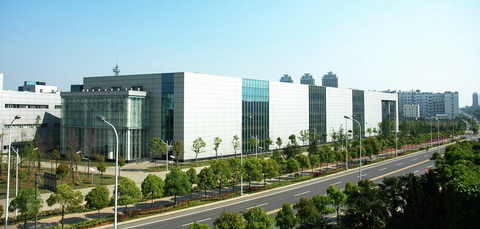
\includegraphics[width=3.5cm]{images/wnlo.jpg}}

\begin{document}

\begin{frame}
	\titlepage
\end{frame}

\begin{frame}
	\frametitle{内容提要}
	\tableofcontents
\end{frame}

\section{第二讲}
\begin{frame}
	\frametitle{第二讲 感知和认知基础}
	\begin{itemize}
		\item 人的感知
		\item 认知过程与交互设计原则
		\item 概念模型及认知
		\item 分布式认知
	\end{itemize}
\end{frame}

\subsection{人的感知}
\begin{frame}
	\frametitle{人的感知}
	\beamertemplatetransparentcovereddynamicmedium 
	\begin{itemize}[<+->]
		\item 人的感知即\textbf{通过人体器官和组织进行人与外部世界的信息的交流和传递}
		\item 认知是人们在进行日常活动时发生于头脑中的事情
		\begin{itemize}
			\item 涉及思维、记忆、学习、幻想、决策、看、读、写和交谈等
		\end{itemize}
		\item 人的感知是认知的基础,认知是将感知获取的信息综合运用
		\begin{itemize}
			\item 认知分为\textbf{经验认知}和\textbf{思维认知}
			\item 认知过程是相互联系的,单纯的一个认知过程是非常少见的
		\end{itemize}
	\end{itemize}
\end{frame}

\begin{frame}
	\frametitle{认知心理学 Cognitive Psychology}
	\beamertemplatetransparentcovereddynamicmedium 
	\begin{itemize}
		\item 认知心理学是二十世纪50年代中期在西方兴起的一种心理学思潮,二十世纪70年代开始其成为西方心理学的一个主要研究方向。\pause
		\item 是构成人类行为基础的心理机制,其核心是输入和输出之间发生的内部心理过程。\pause
		\item 与西方传统哲学也有一定联系,其主要特点是\textbf{强调知识的作用,认为知识是决定人类行为的主要因素}。\pause
		\item 认知心理学研究:
		\begin{itemize}
			\item 人们如何获得外部世界信息
			\item 信息在人脑内如何表示并转化为知识
			\item 知识怎样存储又如何用来指导人们的注意和行为
		\end{itemize}
	\end{itemize}
\end{frame}

\begin{frame}
	\frametitle{感知通道}
	\beamertemplatetransparentcovereddynamicmedium 
	\begin{itemize}
		\item \onslide<1->{五种基本感知的绝对阈限:}
		\begin{itemize}
			\item \textbf{视觉}: \onslide<2->{在黑暗而空气清新的夜晚, 人们可以看到48公里外的一只烛光;} 
			\item \textbf{听觉}: \onslide<3->{在安静的环境中, 人能够听到6米远处的手表滴答声;}
			\item \textbf{嗅觉}: \onslide<4->{人能嗅到1公升空气中散布的1/10万毫克的人造麝香的气味; }
			\item \textbf{味觉}: \onslide<5->{人可尝出9升水中放一茶匙糖的甜味; }
			\item \textbf{触觉}: \onslide<6->{人可感到蜂蜜翅膀距脸颊1厘米处落下。}
		\end{itemize}
	\end{itemize}
\end{frame}

\begin{frame}
	\frametitle{视觉感知}
	\beamertemplatetransparentcovereddynamicmedium 
	\begin{itemize}[<+->]
		\item 外界\textbf{80\%的信息}都是通过视觉得到的,视觉是人与周围世界发生联系的最重要的感觉通道。
		\item 视觉显示是人机交互系统中用的最多的人机界面。
		\item 视觉感知两阶段:\textbf{受到外部刺激接收信息阶段}和\textbf{解释信息阶段}。
	\end{itemize}	
\end{frame}

\begin{frame}
	\frametitle{视觉感知~{\small 特点}}
	\beamertemplatetransparentcovereddynamicmedium
	\transwipe
	\setbeamercolor{uppercol}{fg=white,bg=green!80!gray}
	\setbeamercolor{lowercol}{fg=black,bg=green!20!white}
	\begin{columns}
		\column{5cm}
		\onslide<1->{
			\begin{beamerboxesrounded}[upper=uppercol,lower=lowercol,shadow=true]{受到外部刺激接收信息}
				眼睛和视觉系统的物理特性决定了人类无法看到某些事物
			\end{beamerboxesrounded}
		}
		\column{5cm}
		\onslide<2->{
			\begin{beamerboxesrounded}[upper=uppercol,lower=lowercol,shadow=true]{解释信息}
				视觉系统进行解释处理信息时可对不完全信息发挥一定的想象力
			\end{beamerboxesrounded}
		}
	\end{columns}
	~\\
	\onslide<3->{进行人机交互设计需要清楚这两个阶段及其影响,了解人类真正能够看到的信息。}
\end{frame}

\begin{frame}
	\frametitle{眼睛的构造}
	\transboxout
	\begin{center}
		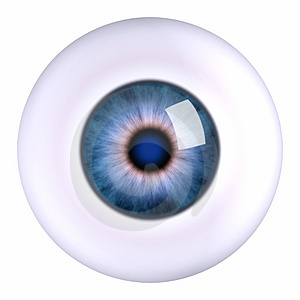
\includegraphics[width=6cm]{images/eyeball.jpg}
	\end{center}
\end{frame}

{% big blank frame with image inside, \(b/e)group can also be used here
\usebackgroundtemplate{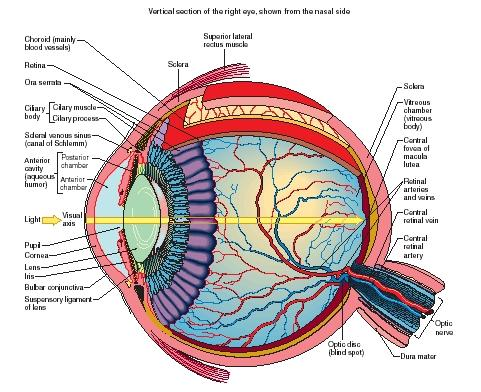
\includegraphics[width=\paperwidth]{images/eyeball-anatomy.jpg}}
\frame[plain]{\transdissolve}
}

\begin{frame}
	\frametitle{视干细胞和视锥细胞}
	\beamertemplatetransparentcovereddynamicmedium
	\begin{tabular}[t]{p{4.5cm}|p{4.5cm}}
		\hline
		视干细胞 & 视锥细胞\\\hline
		在低水平照明时起作用 & 在高水平照明时起作用\\\hline
		区别黑白 & 区别彩色\\	\hline
		对光谱中绿色部分最敏感 & 对光谱中黄色部分最敏感\\\hline
		在远离视网膜中心处最多 & 在视网膜中部最多\\\hline
		对极弱的刺激敏感 & 识别空间位置、敏锐地看物体\\\hline
	\end{tabular}
\end{frame}

\begin{frame}
	\frametitle{视角和视敏度}
	\beamertemplatetransparentcovereddynamicmedium
	\begin{columns}
		\column{7.5cm}
		\begin{center}
			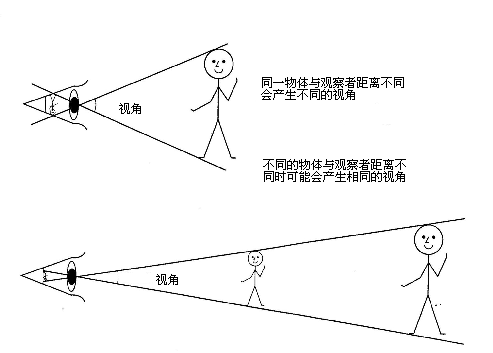
\includegraphics[width=5cm]{images/viewport.png}
		\end{center}
		\begin{itemize}[<+->]
			\item 视敏度:{\tiny 指人眼对细节的感知能力,通常用被辨别物体最小间距所对应的视角的倒数表示。通常将能分辨出视角1′的视敏度定为1.0。}
			\item 一般人能够在2m的距离分辨2mm-20mm的间距,为我们设计界面时字符大小和间距提供了依据
		\end{itemize}
	\column{2.5cm}
	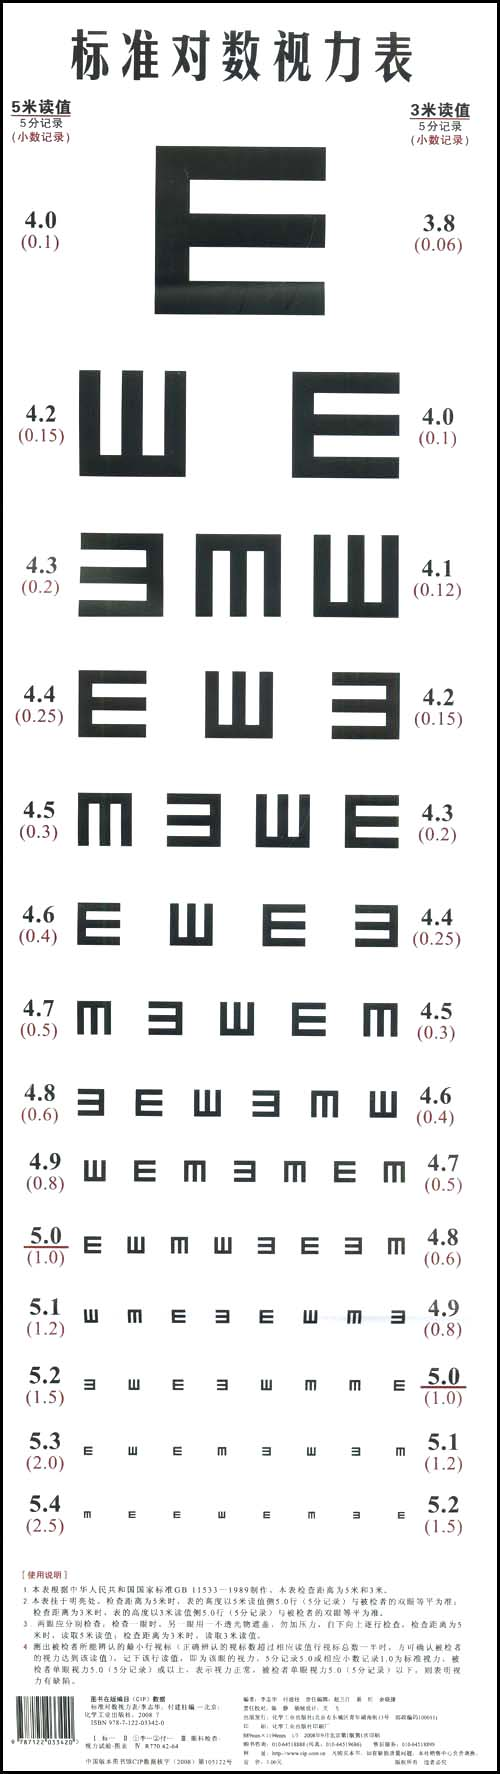
\includegraphics[width=2cm]{images/eye-chart.jpg}
	\end{columns}
\end{frame}

\begin{frame}
	\frametitle{感知物体大小、相对距离和深度}
	\beamertemplatetransparentcovereddynamicmedium
	\begin{columns}
	\column{5cm}
	利用视觉影像中的线索:
	\begin{itemize}
		\item<1-> 覆盖关系\\{\tiny 被覆盖的物体相对较远;}
		\item<2-> 大小比例\\{\tiny 一般来讲,较大的物体距离较近;}
		\item<3-> 对物体的熟悉度\\{\tiny 对非常熟悉物体,人们对物体的大小在头脑中事先有一个期望和预测,因此在判断物体距离时很容易和他看到的物体的大小联系起来。} 
	\end{itemize}
	\column{5cm}
	\begin{center}
		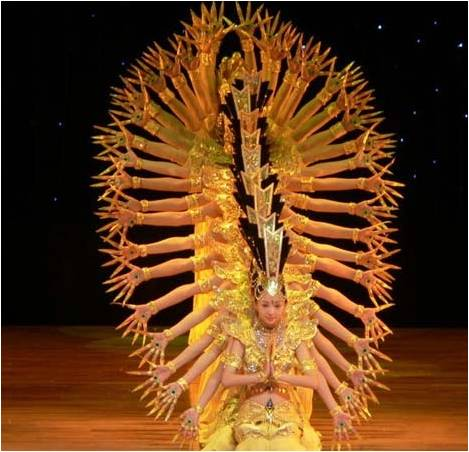
\includegraphics[width=4cm]{images/depth.jpg}
	\end{center}
	\end{columns}
\end{frame}

\begin{frame}
	\frametitle{感知亮度及色彩}
	\beamertemplatetransparentcovereddynamicmedium
	\begin{center}
		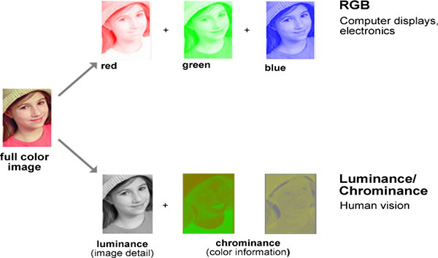
\includegraphics[width=6cm]{images/04_rgb_luminance.jpg}
	\end{center}
%	\begin{itemize}
%		\item 亮度是光线明亮程度的主观反映 
%		\item 增强亮度可以提高视敏度 
%		\item 随着亮度的增加,闪烁感也会增强。~在高亮度时,光线变化低于50Hz,视觉系统就会感到闪烁
%	\end{itemize}
%	\begin{itemize}
%		\item 人能感觉到不同的颜色,这是眼睛接受不同波长的光的结果。 
%		\item 颜色通常用三种属性表示:色度、强度和饱和度。
%		\item 色度是由光的波长决定的,正常的眼睛可感受到的光谱波长为400μm-700μm。
%	\end{itemize}
	\begin{itemize}[<+->]
		\item 视敏度影响、闪烁感与50Hz界限
		\item 波长,可视光谱,三种属性:\\{\tiny 色度 chrominance、强度 luminance 和饱和度 saturation}
		\item 在设计交互界面时,要\textbf{考虑使用者对亮度、闪烁以及色彩对比的感知},避免疲劳,创造舒适的交互环境。
	\end{itemize}
\end{frame}

\begin{frame}
	\frametitle{视觉行为的整体性~{\small 格式塔 (Gestalt) 心理学}}
	Gestalt(德): ``模式、形状、形式''\\即``动态的整体(dynamic wholes)''
	\begin{center}
	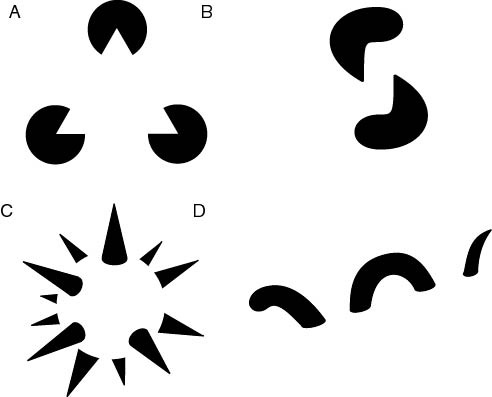
\includegraphics[width=5cm]{images/Reification.jpg}~
\includegraphics[width=5cm]{images/744px-Multistability.svg.png}\\
	\end{center}
	{\tiny http://zh.wikipedia.org/wiki/格式塔学派}
\end{frame}

\begin{frame}
	\frametitle{视错觉~{\small 莱亚错觉 Müller-Lyer illusion}}
	\begin{center}
	\begin{tikzpicture}
		\onslide<1>{
			\draw (1,1) -- (0,0); \draw (1,1) -- (0,2); \draw (6,1) -- (7,0);  \draw (6,1) -- (7,2);
			\draw (1,4) -- (2,3); \draw (1,4) -- (2,5); \draw (6,4) -- (5,3);  \draw (6,4) -- (5,5);
		}
		\onslide<1,2>{
			\draw (1,1) -- (6,1);
			\draw (1,4) -- (6,4);
		}
	\end{tikzpicture}
	\end{center}
%	http://en.wikipedia.org/wiki/Müller-Lyer_illusion
\end{frame}

\begin{frame}
	\frametitle{视错觉~{\small 艾宾浩斯错觉 Ebbinghaus illusion}}
	\begin{center}
	\begin{tikzpicture}
		\onslide<1>{
			\foreach \c in {(1,0), (0,1), (2,1), (1,2)} \fill \c + (0.5,0.5) circle (0.50);
			\foreach \c in {(6,0), (5,1), (7,1), (6,2)} \fill \c + (0.5,0.5) circle (0.30);
		}
		\onslide<1,2>{
			\foreach \c in {(1,1)} \fill \c + (0.5,0.5) circle (0.40);
			\foreach \c in {(6,1)} \fill \c + (0.5,0.5) circle (0.40);
		}
	\end{tikzpicture}
	\end{center}
%	http://en.wikipedia.org/wiki/Ebbinghaus_illusion
\end{frame}

\begin{frame}
	\frametitle{视错觉~{\small 弗雷泽图形 Fraser spiral illusion}}
	\begin{center}
	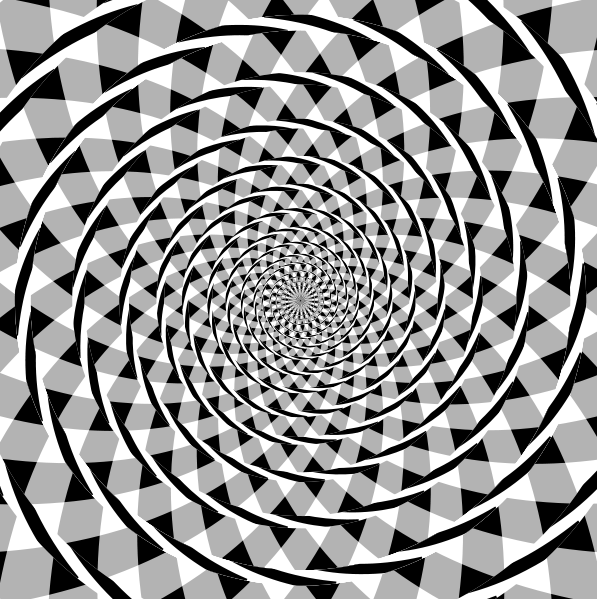
\includegraphics[width=6cm]{images/597px-Fraser_spiral.svg.png}\\
	\end{center}
%	http://en.wikipedia.org/wiki/Fraser_spiral_illusion
\end{frame}

\begin{frame}
	\frametitle{视错觉~{\small 静止图像的运动}}
	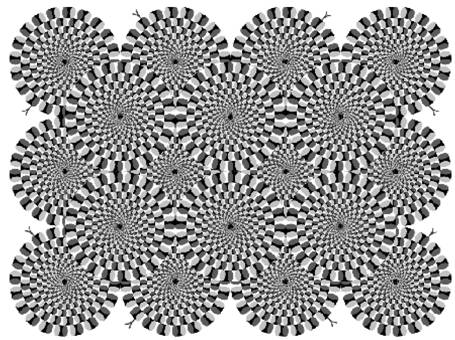
\includegraphics[width=9cm]{images/illusion1.jpg}
\end{frame}

% http://news.bbc.co.uk/2/hi/uk_news/england/north_yorkshire/7610761.stm
% The University of York's Psychology Department asked people to decide which women wearing striped dresses looked slimmer in 200 pairs of pictures.
\begin{frame}
	\frametitle{视觉行为影响}
	\transwipe
	\begin{center}
		
\includegraphics[width=8cm]{images/bar_comparison.jpg}\\\pause
		\begin{beamerboxesrounded}[shadow=true]{Dr. Peter Thompson}
			\textit{``Horizontal stripes don't make you look fat''}
		\end{beamerboxesrounded}
	\end{center}
\end{frame}

\begin{frame}
	\frametitle{视觉行为影响}
	\transwipe
	\begin{center}
	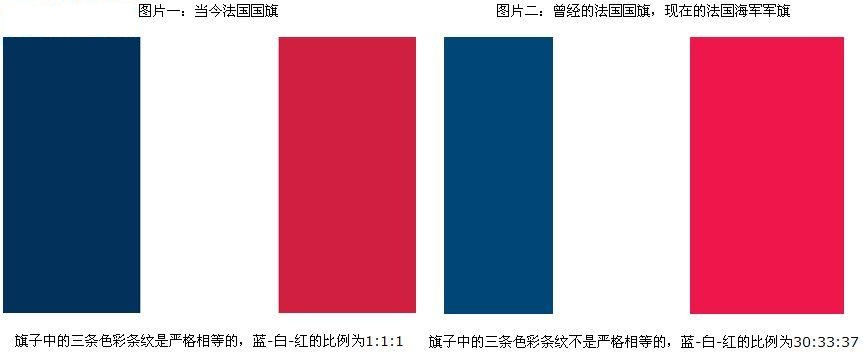
\includegraphics[width=8cm]{images/flag_comparison.jpg}
	\end{center}
\end{frame}

\begin{frame}
	\frametitle{视觉行为影响}
	\beamertemplatetransparentcovereddynamicmedium
	\begin{itemize}
		\item 物体的组合方式将影响观察者的感知方式:
		\begin{itemize}[<+->]
			\item 人们总会夸大水平线而缩短垂直线。
			\item 视错觉同样会影响到显示页面的对称性。
			\item 人们经常把对称页面的中心看得稍微偏上些\\{\tiny 如果页面以实际中心为基准排版设计,人们就会感到页面上部比下部分要短,影响视觉效果}。
			\item 在实际设计过程中,设计者应\textbf{以视觉中心为基准}设计图形界面。
		\end{itemize}
	\end{itemize}
\end{frame}


\begin{frame}
	\frametitle{阅读}
	\beamertemplatetransparentcovereddynamicmedium
	\begin{itemize}
		\item 进行交互界面设计时,文字符号的处理,特别是文字的排版和显示,也要根据人们的视觉感知特点,找出其中一些规律。\pause
		\item 阅读分为几个阶段:
		\begin{itemize}
			\item 页面上文字的形状被人眼感知
			\item 文字被编码成相关的内部语言表示
			\item 语言在人脑中被解释成有语法和语义的单词或句子
		\end{itemize}\pause
		\item 成年人阅读是通过字的特征(如字的形状)加以识别。\\{\tiny 改变字的显示方式(如用大写字母,改变字体等),会影响到阅读的速度和准确性。}
	\end{itemize}
\end{frame}

\begin{frame}
	\frametitle{阅读~{\small 舒适性}}
	\beamertemplatetransparentcovereddynamicmedium
	\begin{center}
		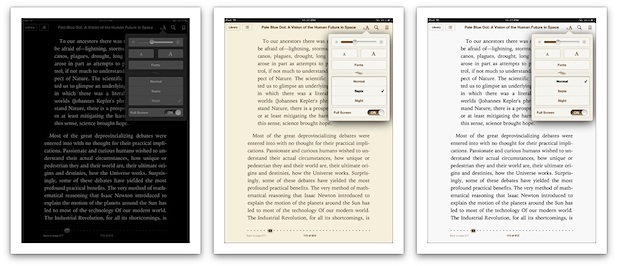
\includegraphics[width=9cm]{images/ibooks-themes.jpg}
	\end{center}
	\begin{itemize}
		\item 9~12号的标准字体(英文)\pause
		\item 页面的宽度在58~132mm之间\pause
		\item 在明亮的背景下显示灰暗的文字 VS. 灰暗的背景下显示明亮的文字
	\end{itemize}
\end{frame}

\begin{frame}
	\frametitle{颜色模型~{\small RGB, CMYK}}
	% 动机,主动光源显示(显示器)与被动反射(印刷)
	\begin{center}
	\begin{tikzpicture}[scale=.5]
	% Create the background in the circle, by drawing several slices
	% each with a constant color given by the angle (which is converted
	% to a color usin the hue, saturation and brightness color space).
%	\foreach \x in {0,0.0111,...,1} {
%		\definecolor{currentcolor}{hsb}{\x, 1, 1}
%		\draw[draw=none, fill=currentcolor]
%			(-360*\x+88:2) -- (-360*\x+88:3.8)
%			-- (-360*\x+92:3.8) -- (-360*\x+92:2) -- cycle;
%	}

	% On top of the background draw three spotlights of the primary colors
	% red, green and blue (they are primary in an additive colorspace where
	% light are mixed)
	\draw [draw=none, fill=red] (90:1.5) circle (2cm);
	\draw [draw=none, fill=green] (-30:1.5) circle (2cm);
	\draw [draw=none, fill=blue] (210:1.5) circle (2cm);
	
	% Draw areas where two of the three primary colors are overlapping.
	% These areas are the secondary colors yellow, cyan and magenta.
	\begin{scope} % red + green = yellow
		\clip (90:1.5) circle(2cm);
		\draw [draw=none, fill=yellow] (-30:1.5) circle (2cm);
	\end{scope} % blue + red = magenta
	\begin{scope}
		\clip (210:1.5) circle(2cm);
		\draw [draw=none, fill=magenta] (90:1.5) circle (2cm);
	\end{scope}
	\begin{scope} % green + blue = cyan
		\clip (-30:1.5) circle(2cm);
		\draw [draw=none, fill=cyan] (210:1.5) circle (2cm);
	\end{scope}
	
	% Draw the center area which consists of all the primary colors.
	\begin{scope} % red + green + blue = white
		\clip (90:1.5) circle(2cm);
		\clip (210:1.5) circle(2cm);
		\draw [draw=none, fill=white] (-30:1.5) circle (2cm);	
	\end{scope}

	% Draw a circle with markings along the perimeter, indicating which angles
	% the hue function connects to certain colors.
	\draw (0, 0) circle (3.9cm);
	\foreach \x  in {0, 30, ..., 330}
		\draw (-\x+90:3.8) -- (-\x+90:4.0) (-\x+90:4.4) node {$\x^\circ$};

	% Add labels with names of the primary and secondary colors.
	\foreach \x/\text in {0/red, 60/yellow, 120/green, 180/cyan, 240/blue, 300/magenta}
		\draw (-\x+90:5.5) node {\text};
	\end{tikzpicture}
	\end{center}
\end{frame}

\begin{frame}
	\frametitle{颜色模型~{\small HSV}}
	Hue(色相)、Saturation(饱和度)和Value(值或明度)
	% 红、绿、蓝分别相隔120度。互补色分别相差180度。
	% 纯度S为一比例值,范围从0到1,它表示成所选颜色的纯度和该颜色最大的纯度之间的比率。
	% S=0时,只有灰度。
	% V表示色彩的明亮程度,范围从0到1。
	% 有一点要注意:它和光强度之间并没有直接的联系。
	% 动机:色彩形成与生物识别机制之关联
	\begin{center}
		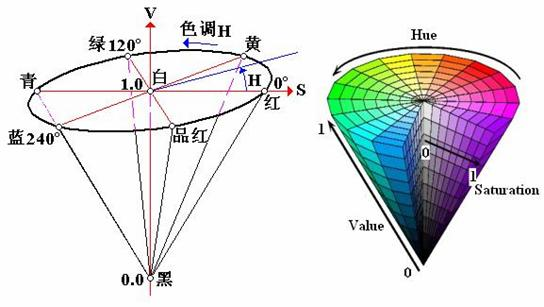
\includegraphics[width=8cm]{images/HSV_ColorModel.jpg}
	\end{center}
\end{frame}

\begin{frame}
	\frametitle{听觉}
	\beamertemplatetransparentcovereddynamicmedium 
	\begin{itemize}[<+->]
		\item 听觉感知传递的信息仅次于视觉,可人们一般都低估了这些信息。\\{\small 人的听觉可以感知大量的信息,但被视觉关注掩盖了许多。}
		\item 听觉所涉及的问题和视觉一样,即\textbf{接受刺激,把它的特性转化为神经兴奋,并对信息进行加工,然后传递到大脑}。
	\end{itemize}
\end{frame}

{
\usebackgroundtemplate{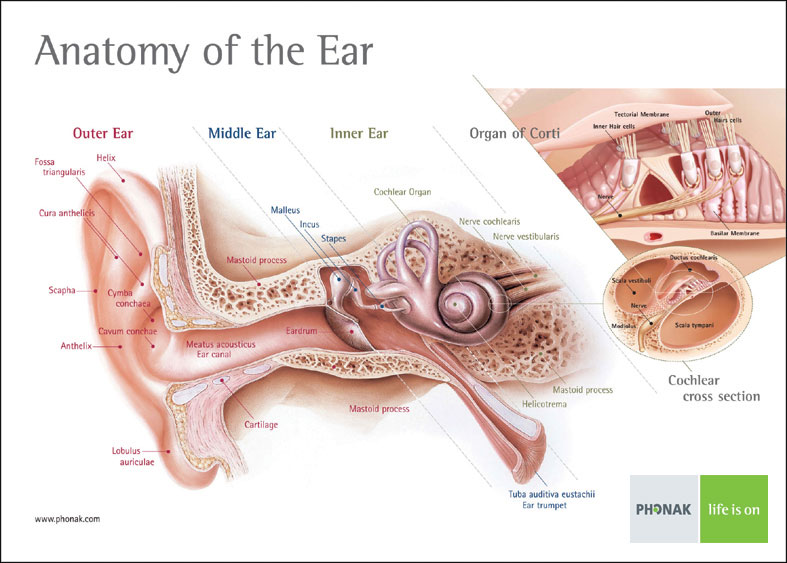
\includegraphics[width=\paperwidth]{images/ear_anatomy_large.jpg}}
\frame[plain]{\transdissolve}
}

\begin{frame}
	\frametitle{声音的处理}
	\beamertemplatetransparentcovereddynamicmedium 
	\begin{itemize}
		\item 声波在空气中的振动传播的特性
		\begin{itemize}
			\item 音调与声波的频率有关,低频能产生低调的声音,高频能产生高调的声音。
			\item 响度指在频率一定的情况下声波的振幅。
			\item 音色与发声的材料有关,不同的乐器可以产生相同频率和振幅的声波,但音色不同。
		\end{itemize}\pause
		\item 人类能够听到频率在20Hz~20kHz之间的声音
		\begin{itemize}
			\item 在1000Hz~4000Hz范围内听觉的感受性最高;
			\item 人可以辨认的语音频率范围是260~5600Hz。
			\item 500Hz以下和5000Hz以上的声音,强度很大时才能被听到。
		\end{itemize}\pause
		\item 响度超过140dB时,所引起的不再是听觉而是痛觉。
	\end{itemize}
\end{frame}

\begin{frame}
	\frametitle{声音的解释}
	\beamertemplatetransparentcovereddynamicmedium 
	\begin{itemize}[<+->]
		\item 听觉系统把输入分为三类:
		\begin{itemize}
			\item 噪声和可以忽略的不重要的声音;
			\item 被赋予意义的非语言声音,如动物的叫声;
			\item 用来组成语言的有意义的声音。
		\end{itemize}
	\end{itemize}
\end{frame}

\begin{frame}
	\frametitle{声音的解释}
	\beamertemplatetransparentcovereddynamicmedium 
	\begin{itemize}
		\item 听觉系统就像视觉系统一样,利用以前的经验来解释输入。\pause
		\item Lindsay PH 和 Norman DA 的``材料-驱动'' (Data-Driven) 和``概念-驱动'' (Conceptually-Driven) 过程~\cite{Langley198131}。
		\begin{itemize}
			\item 材料-驱动~{\tiny 对言语材料在感知水平上进行的加工过程,它是由下而上的分析过程。}
			\item 概念-驱动~{\tiny 在理解水平上进行的加工过程,它是由上而下(从最高的结构概念开始)的分析过程。}
		\end{itemize}\pause
		\item 人类听觉系统对声音的解释可帮助设计人机交互界面中的语音界面
		\begin{itemize}
			\item 语音识别 Voice Recognition
			\item 语音合成 Text to Speech
		\end{itemize}
	\end{itemize}
\end{frame}

\begin{frame}
	\frametitle{触觉}
	\beamertemplatetransparentcovereddynamicmedium 
	\begin{columns}
	\column{6cm}
	\begin{itemize}[<+->]
		\item 人-->机 \textbf{Touch}
		\item 机-->人 \textbf{Haptic perception}
		\item 重要性:\\{\small 交互更自然,帮助能力缺陷人士}
	\end{itemize}
	\column{4cm}
	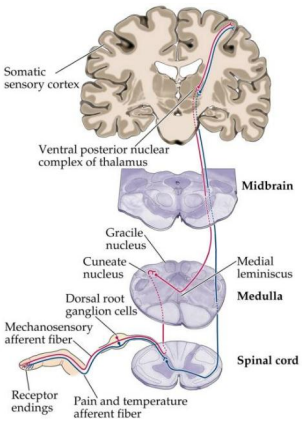
\includegraphics[width=4cm]{images/skin-receptor-path.png}
%	http://wiki.bethanycrane.com/somaticsenses
	\end{columns}
\end{frame}

{
\usebackgroundtemplate{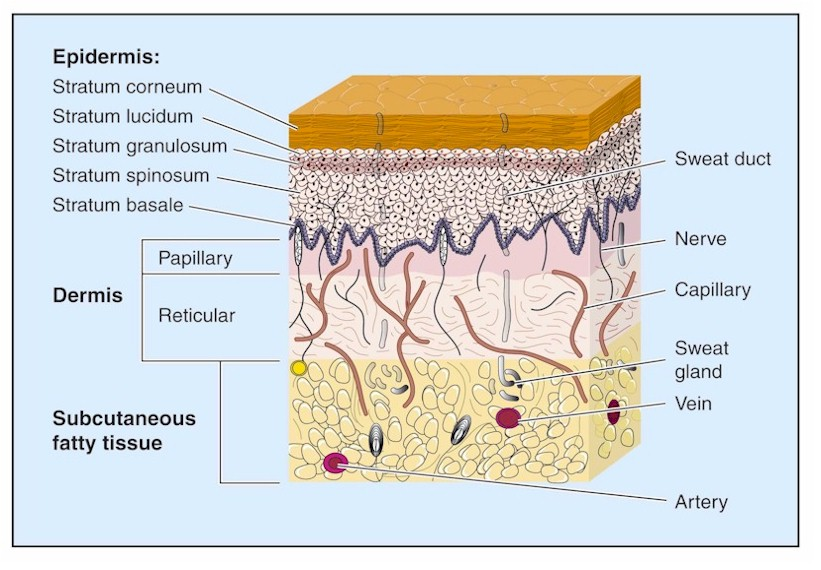
\includegraphics[width=\paperwidth]{images/skin-layers.jpg}}
\frame[plain]{\transdissolve}
}

{
	\usebackgroundtemplate{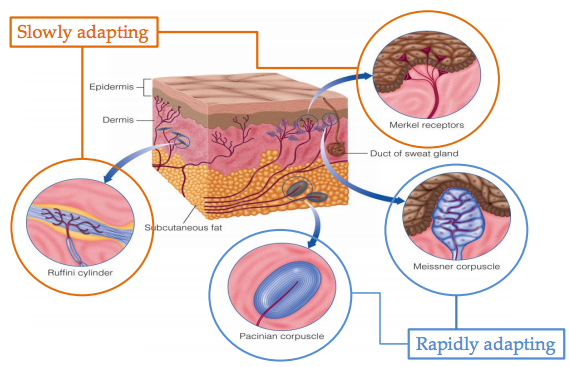
\includegraphics[width=\paperwidth]{images/adapting-fibres.png}}
	\frame[plain]{
		\transdissolve
		\pause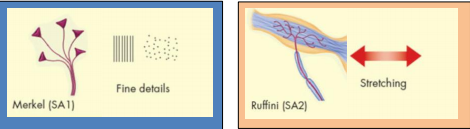
\includegraphics[width=7cm]{images/slowly-adapting-fibres.png}\\~\\
		\pause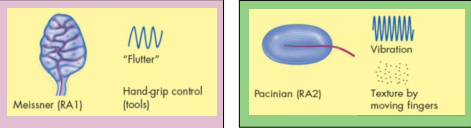
\includegraphics[width=7cm]{images/rapidly-adapting-fibres.png}
	}
}

\begin{frame}
	\frametitle{触觉~{\small 特点}}
	\begin{itemize}
		\item 触觉的感知机理与视觉和听觉的最大不同在于它的非局部性
		\begin{itemize}
			\item \textbf{冷热}~温度感受
			\item \textbf{疼痛}~伤害感受
			\item \textbf{压力}~机械刺激感受
		\end{itemize}
	\end{itemize}
	\transdissolve\pause
	\begin{center}
		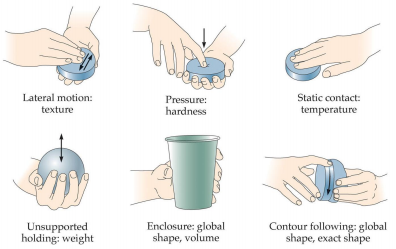
\includegraphics[scale=.5]{images/tactile-sensitivity.png}
	\end{center}
\end{frame}

\begin{frame}
	\frametitle{触觉}
	\begin{itemize}
		\item 实验表明,人手指的触觉敏感度是前臂的触觉敏感度的10倍。
		\item 对人身体各部位触觉敏感程度的了解有助于基于触觉的交互设备的设计。
%		\item 动觉:对人的躯干和四肢的位置的感觉,主要由于人的关节处的感受器。
	\end{itemize}
\end{frame}

\subsection{认知过程与交互设计原则}
\begin{frame}
	\frametitle{认知过程与交互设计原则}
	\begin{columns}
		\column{4cm}
		\onslide<2>{许多认知过程是相互依赖的,一个活动可同时涉及多个不同的过程。}
		\column{6cm}
		\begin{tikzpicture}
			[node distance=.3cm, start chain=going below,]
	  		\node[punktchain, join] (a) {感知和识别};
			\node[punktchain, join] (b) {注意};
			\node[punktchain, join] (c) {记忆};
			\node[punktchain, join] (d) {学习};
			\node[punktchain, join] (e) {阅读};
			\node[punktchain, join] (f) {说话和聆听};
			\node[punktchain, join] (g) {解题、规划、推理和决策};
		\end{tikzpicture}
	\end{columns}
\end{frame}

{
\usebackgroundtemplate{
\includegraphics[width=\paperwidth, height=\paperheight]{images/focus.jpg}}
\frame[plain]{\transdissolve}
}

\begin{frame}
	\frametitle{注意}
	\transdissolve
	\begin{columns}
		\column{5cm}
		\begin{itemize}
			\item 注意\\{\tiny 在某个时刻,从众多可能的事物中选择一个,并把精力集中在这个事物上。} 
			\item 注意的不同类型
			\begin{itemize}
				\item 视觉关注
				\item 听觉关注
			\end{itemize}		
			\item 注意相关的因素
			\begin{itemize}
				\item 目标
				\item 信息的表示形式
			\end{itemize}		
		\end{itemize}
		\column{5cm}
		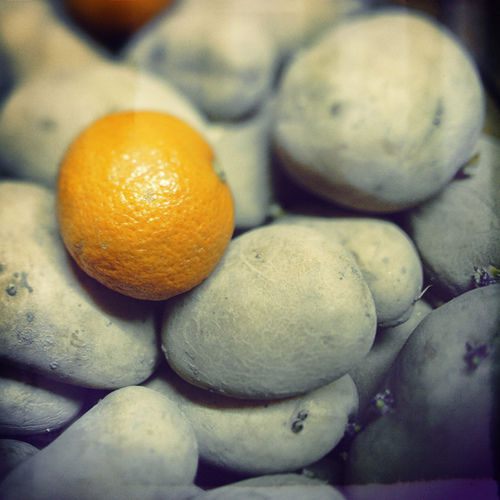
\includegraphics[width=4cm]{images/focus1.jpg}\\
		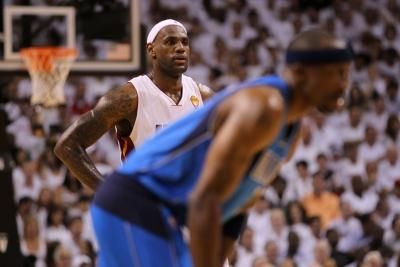
\includegraphics[width=4cm]{images/focus2.jpg}
	\end{columns}
\end{frame}

\begin{frame}
	\frametitle{信息表示方法}
	\beamertemplatetransparentcovereddynamicmedium 
	\begin{itemize}
		\item 信息的显示方式对于人们能否快速捕捉到所需的信息片断有很大的影响。\pause
		\begin{itemize}
			\item 结构化的信息比较便于人们查找
			\item 图形化的信息比较便于人们理解
			\item 多媒体的信息比较便于人们快速接受
		\end{itemize}	
	\end{itemize}
\end{frame}

% http://www.smashingmagazine.com/2007/08/02/data-visualization-modern-approaches/
{
\usebackgroundtemplate{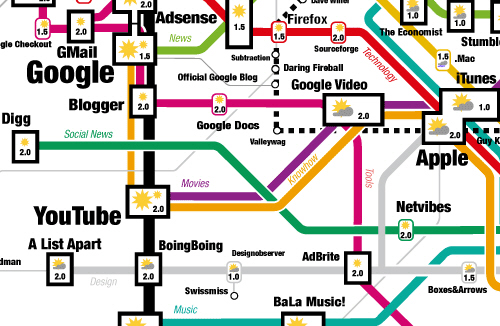
\includegraphics[width=\paperwidth, height=\paperheight]{images/webtrends2007.jpg}}
\frame[plain]{\transdissolve}
}

{
\usebackgroundtemplate{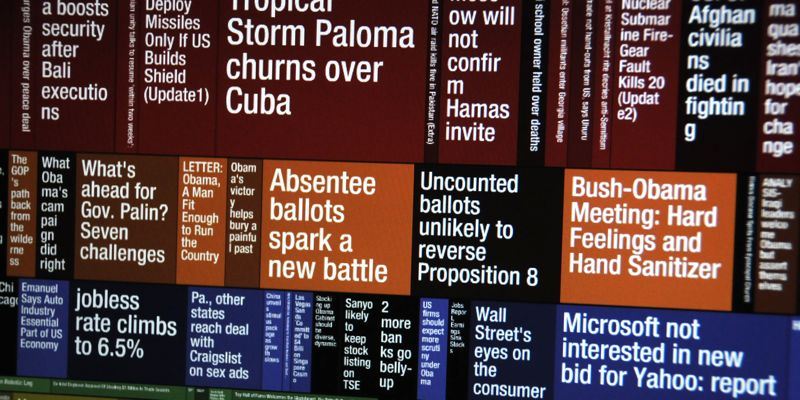
\includegraphics[width=\paperwidth, height=\paperheight]{images/newsmap.jpg}}
\frame[plain]{\transdissolve}
}

{
\usebackgroundtemplate{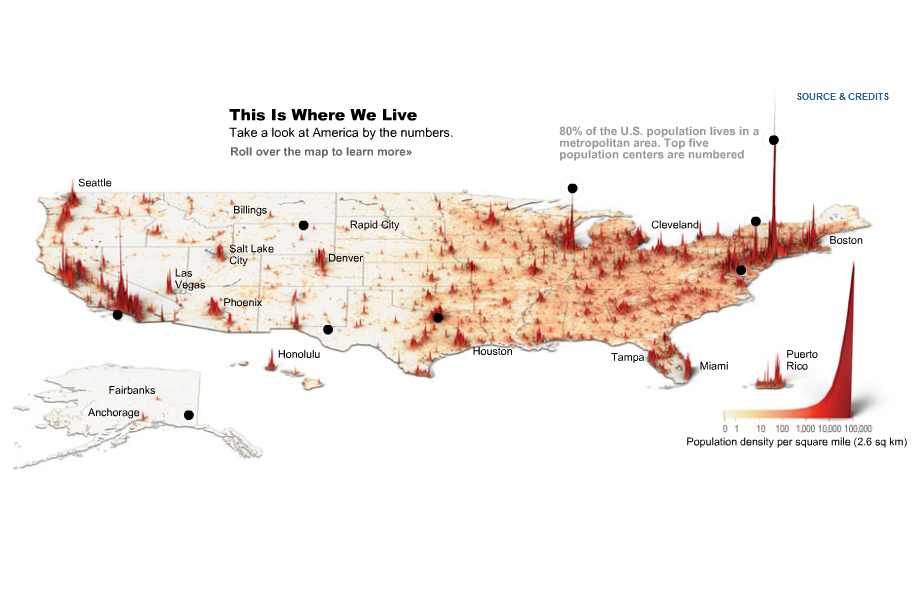
\includegraphics[width=\paperwidth, height=\paperheight]{images/www.time.com-2012-9-10.png}}
\frame[plain]{\transdissolve}
}

% http://www.crazyegg.com/home2
% web heatmap

% http://xiaoji-chen.com/blog/
{
\usebackgroundtemplate{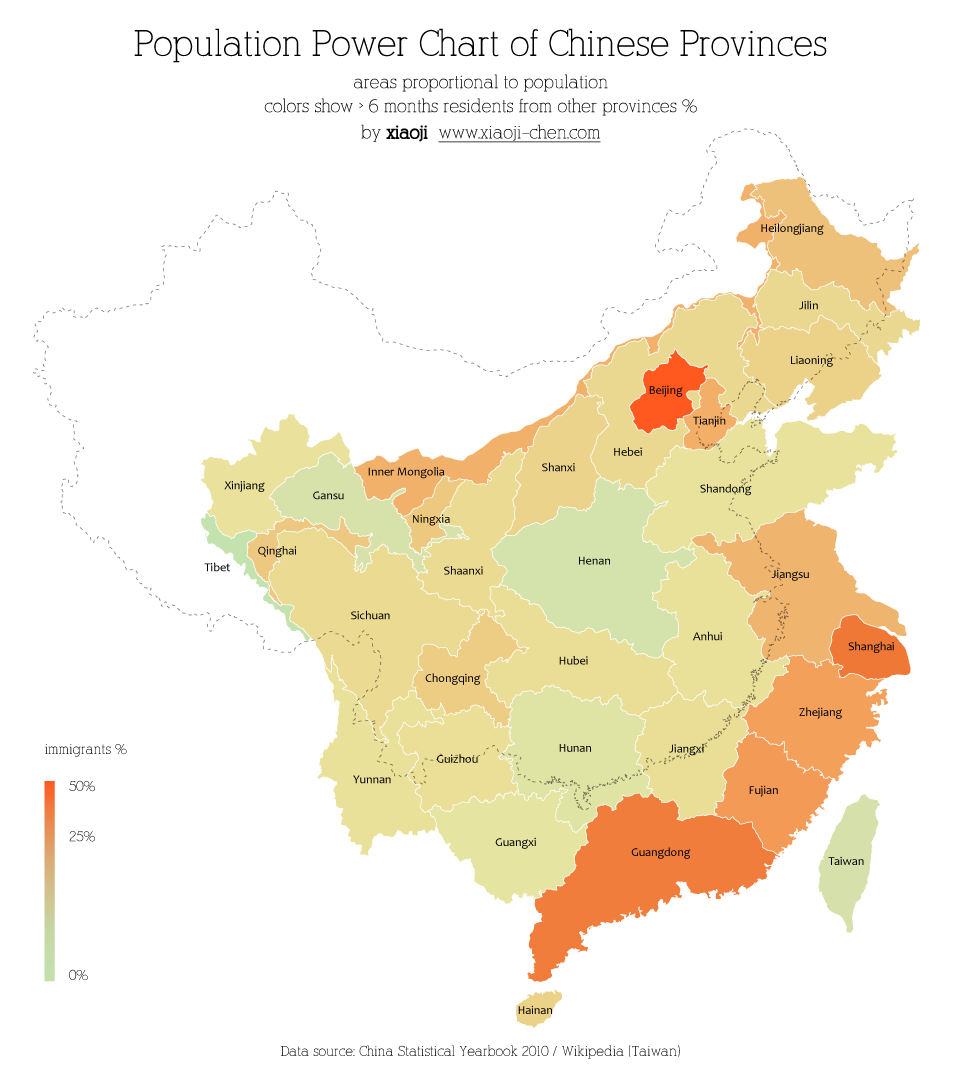
\includegraphics[width=\paperwidth, height=\paperheight]{images/cartogram-02.png}}
\frame[plain]{\transdissolve}
}

{
\usebackgroundtemplate{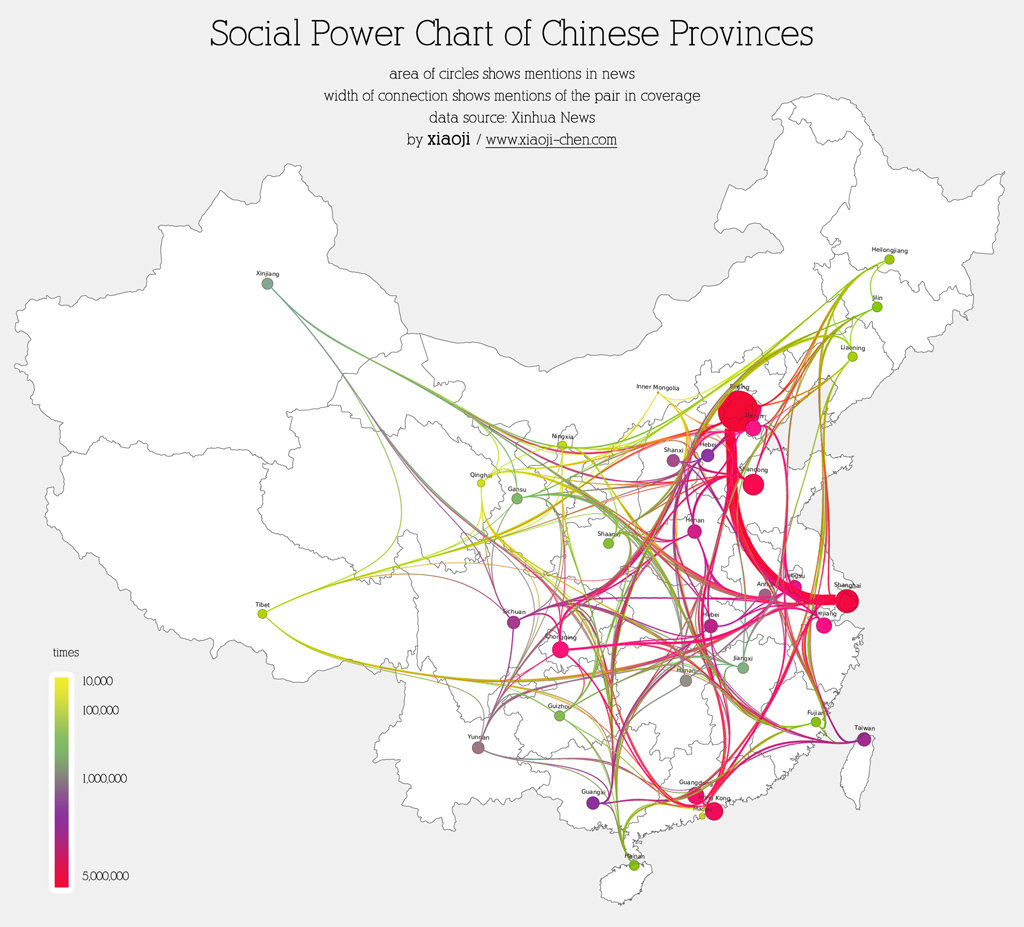
\includegraphics[width=\paperwidth, height=\paperheight]{images/network_en.jpg}}
\frame[plain]{\transdissolve}
}

\begin{frame}
	\frametitle{注意特点对界面设计的要求}
	\beamertemplatetransparentcovereddynamicmedium
	\begin{itemize}
		\item 在设计人机交互界面时应做到
		\begin{itemize}[<+->]
			\item 使重要信息吸引注意
			\item 高亮醒目,运动,色彩,线框,序列 \dots
			\item 朴实,简洁,避免过度拥挤,分散注意,造成疲劳
		\end{itemize}
	\end{itemize}
\end{frame}

% http://www.aharef.info/static/htmlgraph/
{
	\usebackgroundtemplate{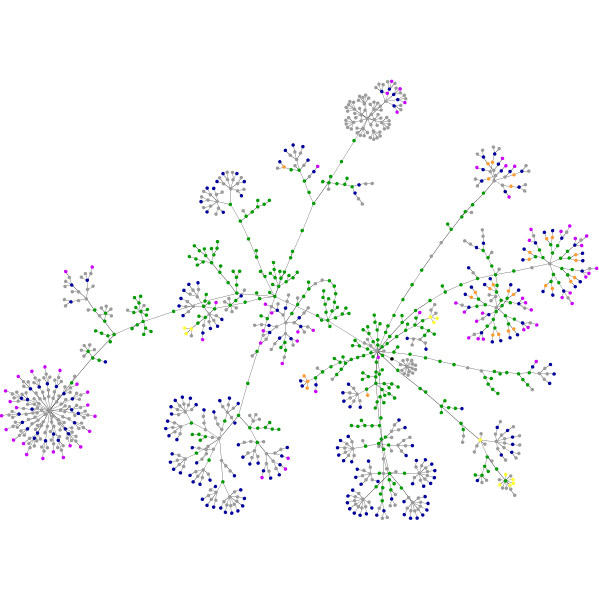
\includegraphics[width=\paperwidth, height=\paperheight]{images/www.aharef.info-2012-9-10-yahoo.png}}
	\begin{frame}[plain]
		\transdissolve
		\onslide<2>{
			\begin{center}
			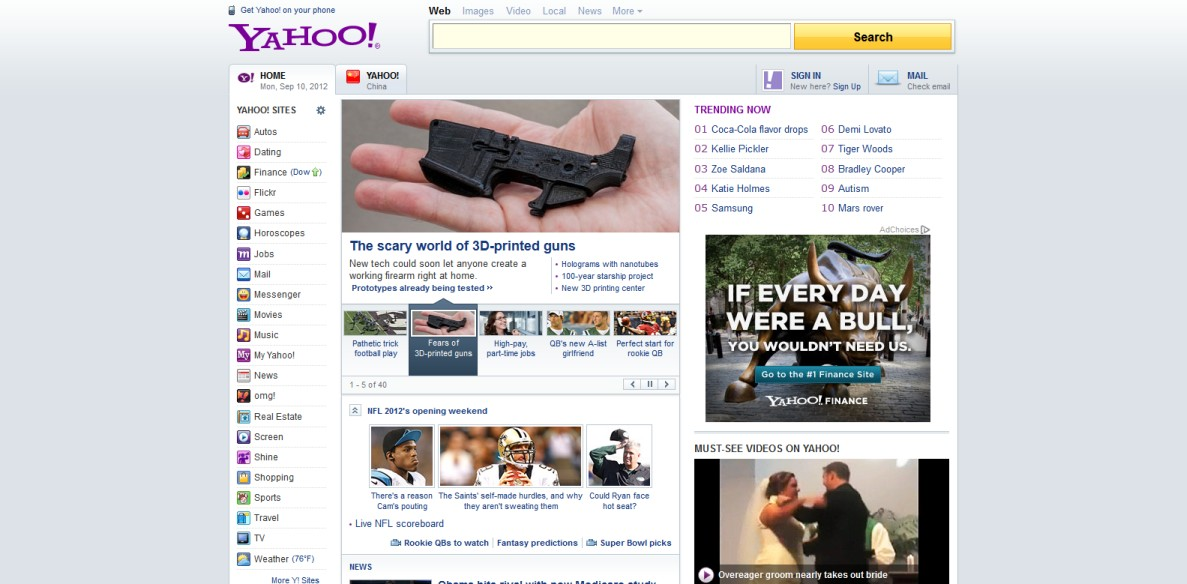
\includegraphics[scale=.3]{images/www.yahoo.com-2012-9-10.jpg}
			\end{center}
		}
	\end{frame}	
}

{
	\usebackgroundtemplate{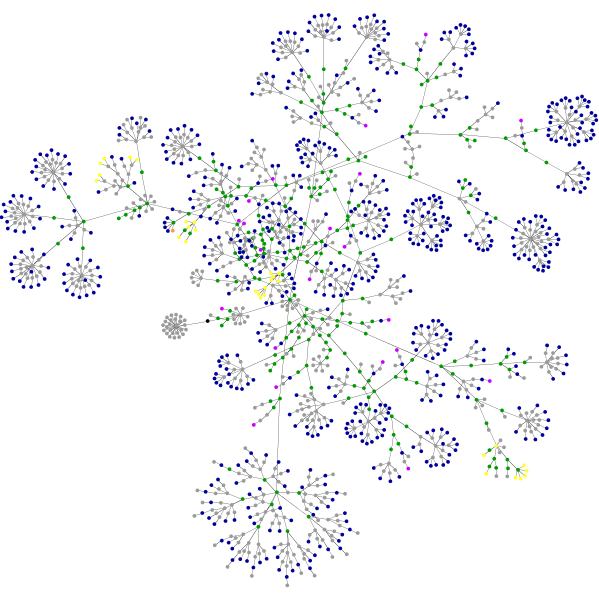
\includegraphics[width=\paperwidth, height=\paperheight]{images/www.aharef.info-2012-9-10-sina.png}}
	\begin{frame}[plain]
		\transdissolve
		\onslide<2>{
			\begin{center}
			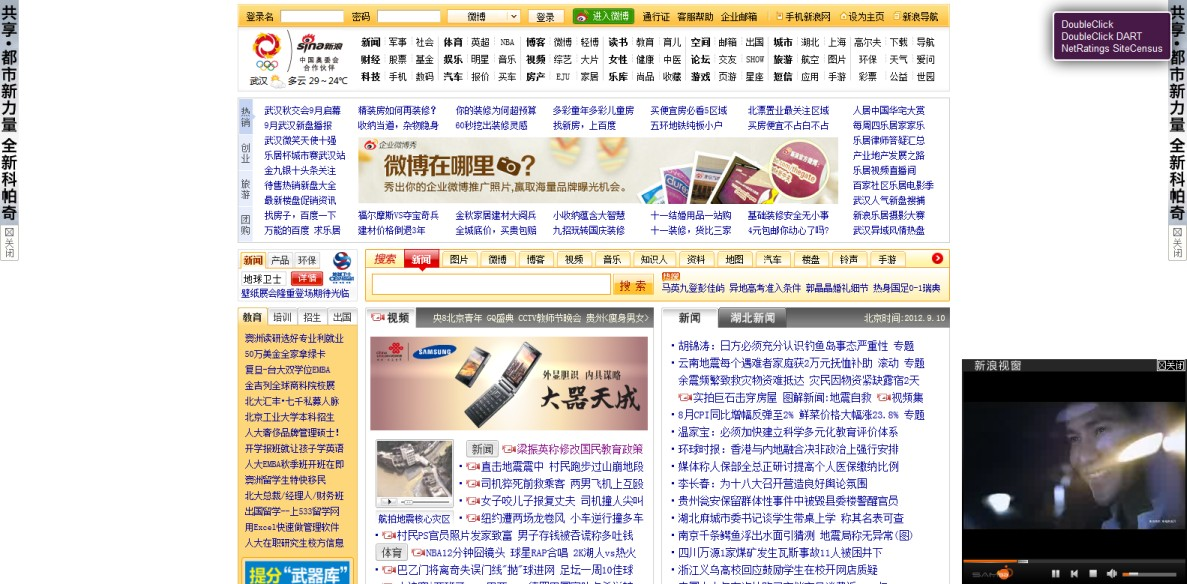
\includegraphics[scale=.3]{images/sina.com.cn-2012-9-10.jpg}
			\end{center}
		}
	\end{frame}	
}

{
	\usebackgroundtemplate{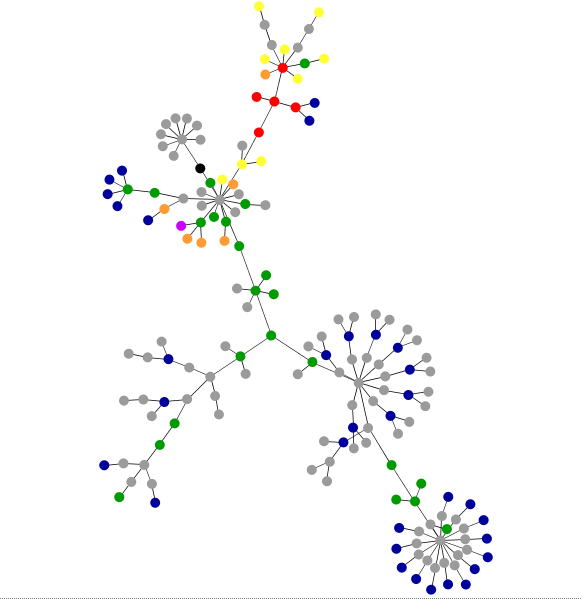
\includegraphics[width=\paperwidth, height=\paperheight]{images/www.aharef.info-2012-9-10-google.png}}
	\begin{frame}[plain]
		\transdissolve
		\onslide<2>{
			\begin{center}
			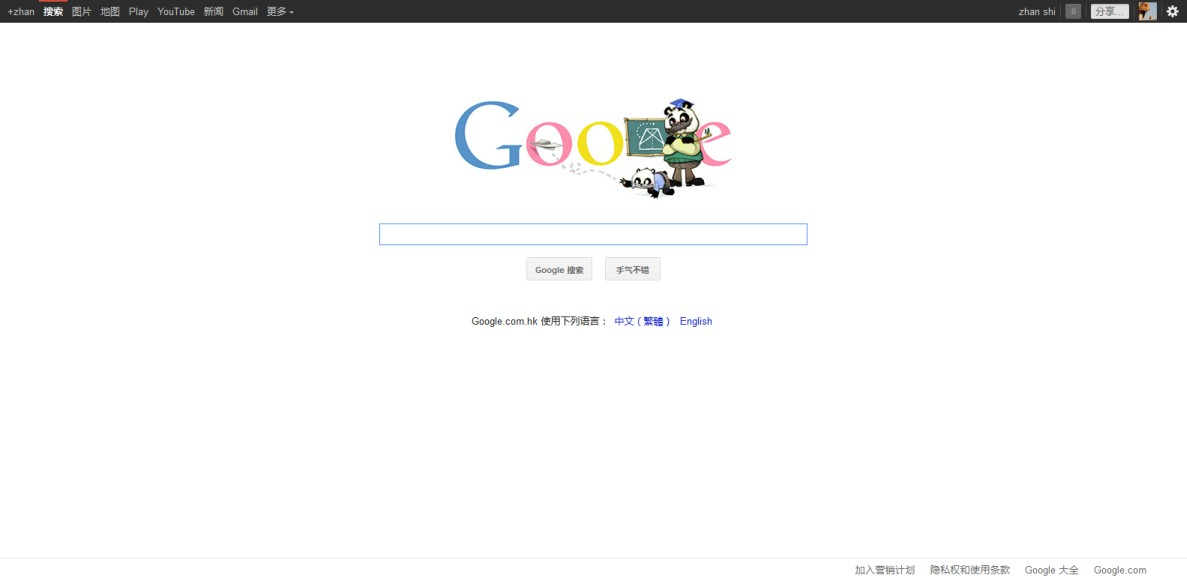
\includegraphics[scale=.3]{images/www.google.com.hk-2012-9-10.jpg}
			\end{center}
		}
	\end{frame}	
}

\begin{frame}
	\beamertemplatetransparentcovereddynamicmedium
	\frametitle{感知和识别}
	\begin{itemize}[<+->]
		\item 在结合不同的媒体时,应确保用户能够理解它们表示的复合信息。
		\item 在结合使用声音和动画时,需要仔细协调,合理安排它们的调用次序。
		\item 用户应能不费力地区别图标或其他图形表示的不同含义。
	\end{itemize}
\end{frame}

\begin{frame}
	\frametitle{记忆}
	\beamertemplatetransparentcovereddynamicmedium
	\begin{itemize}
		\item 回忆各种知识以便采取适当的行动。
		\begin{itemize}[<+->]
			\item \textbf{识记}:相当于信息的输入和编码过程{\tiny ,也就是使不同感官输入的信息,经过编码而成为头脑可接受的形式;}
			\item \textbf{保持}:相当于信息的贮存{\tiny ,即信息在头脑中被再加工整理,使其成为有序地组织结构,以便贮存;}
			\item \textbf{再认和回忆}:再认和回忆相当于信息的提取{\tiny ,编码越完善、组织越有序,提取也就越容易,反之,提取越困难。}
		\end{itemize}
	\end{itemize}
\end{frame}

{
\usebackgroundtemplate{
\includegraphics[width=\paperwidth, height=\paperheight]{images/world-famous-brand-logo-vector-material_15-7097.jpg}}
\frame[plain]{\transdissolve}
}

\begin{frame}
	\frametitle{减轻记忆负担}
	\beamertemplatetransparentcovereddynamicmedium
	\begin{itemize}
		\item 人的识别能力大于回忆能力
		\begin{itemize}
			\item 图文界面替代命令界面
			\item 在线帮助
		\end{itemize}\pause
		\item 回忆提示
		\begin{itemize}
			\item 密码的提示语句
		\end{itemize}
	\end{itemize}
\end{frame}

\begin{frame}
	\frametitle{交互设计原则}
	\beamertemplatetransparentcovereddynamicmedium
	\begin{itemize}[<+->]
		\item 应考虑用户的记忆能力,勿使用过于复杂的任务执行步骤。
		\item 由于用户长于``识别''而短于``回忆'',所以在界面设计应尽量使用菜单、图标,且布局整洁。
		\item 为用户提供多种电子信息(如文件、邮件、图像)的编码方式,并且通过颜色、标志、时间戳、图标等,帮助用户记住它们的存放位置。
	\end{itemize}
\end{frame}

\begin{frame}
	\frametitle{问题解决}
	\beamertemplatetransparentcovereddynamicmedium
	\begin{itemize}[<+->]
		\item 一般步骤:理解问题、制订计划、实施计划、检验结果
		\item 设计中要考虑做什么、有那些选择、执行某个活动会有什么结果?
		\item 人的思维认知能力取决于在相关行业的经验以及对应用和技能的掌握程度。
		\item 在界面中隐藏一些附加信息,供那些希望学习如何更有效地执行任务的用户访问。
	\end{itemize}
\end{frame}

\begin{frame}
	\frametitle{语言处理—阅读、说话、聆听}
	\beamertemplatetransparentcovereddynamicmedium
	\begin{itemize}[<+->]
		\item 听、说、读、写的区别\\{\tiny 外语学习、速度、持续性}
		% 内容严谨性,文字、图形、语音理解速度差别,阅读可重复、聆听不易重复
		\item 语音合成、语音控制须知\\{\tiny ``自然''感受、指令数量}
		% 列队指令、战斗指挥
	\end{itemize}
\end{frame}

\begin{frame}
	\frametitle{影响认知的因素}
	\beamertemplatetransparentcovereddynamicmedium
	\begin{itemize}[<+->]
		\item 情感\\{\tiny 心理状态、情绪影响、情感计算和交流}
		\item 个体\\{\tiny 年龄、性别、身体状态、心智}
		% 摩尔庄园的成功,游戏界面设计
	\end{itemize}
\end{frame}

\subsection{概念模型及认知}
\begin{frame}
	\frametitle{概念模型及认知}
	\begin{center}
		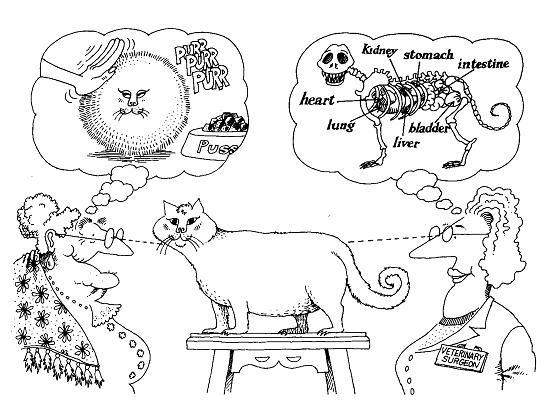
\includegraphics[width=8cm]{images/viewpoint.jpg}
	\end{center}
\end{frame}

\begin{frame}
	\frametitle{概念模型}
	\beamertemplatetransparentcovereddynamicmedium
	\begin{itemize}
		\item 是一种用户能够理解的系统描述,它使用一组集成的构思和概念,描述系统做什么、如何运作、外观如何等。\pause
		\item 设计开发一个概念模型的关键过程包括两个阶段:
		\begin{itemize}
			\item 了解用户任务需求;
			\item 选择交互方式,\\{\tiny 并决定采用何种交互形式(是使用菜单系统,还是使用语音输入,或命令式的系统)。}
		\end{itemize}
	\end{itemize}
\end{frame}

\begin{frame}
	\frametitle{概念模型的迭代开发过程}
	\beamertemplatetransparentcovereddynamicmedium
	\begin{itemize}
		\item 一个完整的概念模型也是一步步充实起来的,可以使用各种方法,包括
		\begin{itemize}
			\item 草拟构思;
			\item 情节串联法;
			\item 描述可能的场景;
			\item 设计原型系统。
		\end{itemize}\pause
		\item 通过不断的与用户交流,逐步完善交互系统的概念模型。
	\end{itemize}
\end{frame}

\begin{frame}
	\frametitle{对概念模型的认知}
	\begin{itemize}
		\item Norman提出了一个用于说明“设计概念模型”与“用户理解模型”之间关系的框架~\cite{norman1988psychology}
		\begin{itemize}
			\item 设计模型——设计师设想的模型,说明系统如何运作。
			\item 系统映像——系统实际上如何运作。
			\item 用户模型——用户如何理解系统的运作。
		\end{itemize}
	\end{itemize}
	\begin{center}
		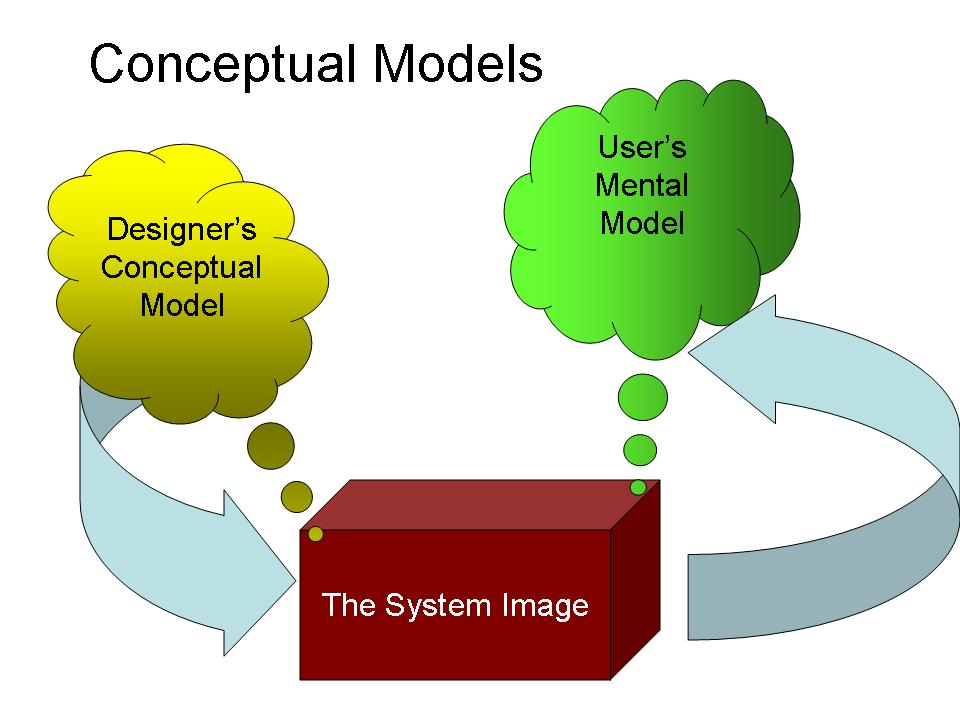
\includegraphics[width=6cm]{images/norman_model.jpg}
	\end{center}
\end{frame}

\begin{frame}
	\frametitle{几种认知概念框架}
	\begin{itemize}
		\item 从人们不同的认知特点,讨论用户如何理解系统概念模型,有:
		\begin{itemize}
			\item 思维模型
			\item 信息处理模型
			\item 外部认知模型
			\item 分布式认知模型
		\end{itemize}
	\end{itemize}
\end{frame}

\begin{frame}
	\frametitle{思维模型}
	\begin{itemize}
		\item 用户思维模型:
		\begin{itemize}
			\item 人们在学习和使用系统的过程中,积累了有关如何使用系统的知识,而且在一定程度上,也积累了有关系统如何工作的知识。
		\end{itemize}
		\item 在认知心理学中,思维模型被认为是外部世界的某些因素在人脑中的反映,掌握和运用思维模型使得人们能够进行推测和推理。
		\item 思维模型牵涉到两个过程—“构建”和“运用”过程\\{\tiny 人们既可能进行有意识的思维处理,也可能进行无意识的思维处理。}
	\end{itemize}
\end{frame}

\begin{frame}
	\frametitle{思维模型用以指导交互的重要性}
	\begin{itemize}
		\item 错误的思维模型带来错误的思维模式
	\end{itemize}
%使用空调调温器(受水龙头、音量控制的影响);
%互联网网页浏览时的错误思维模式。
\end{frame}

\begin{frame}
	\frametitle{正确的思维模型的建立}

\end{frame}

\begin{frame}
	\frametitle{信息处理模型}

\end{frame}

\begin{frame}
	\frametitle{信息处理模型的局限}

\end{frame}

\begin{frame}
	\frametitle{外部认知模型}

\end{frame}

\begin{frame}
	\frametitle{基于外部认知特点的交互式界面设计原则}

\end{frame}

\subsection{分布式认知}
\begin{frame}
	\frametitle{分布式认知模型}
	\beamertemplatetransparentcovereddynamicmedium
	\begin{itemize}
		\item 分布式认知法描述的是认知系统中发生了什么,它通常描述人员之间的交互,人们使用的物品及工作环境。\pause
		\item 例如,要驾驶飞机这个活动涉及:
		\begin{itemize}
			\item 驾驶员、副驾驶员和空中交通管制员之间的交互;
			\item 驾驶员、副驾驶员与驾驶舱内各种仪表的交互;
			\item 驾驶员、副驾驶员与飞机所处环境的交互,如空中航线、跑道。
		\end{itemize}\pause
		\item 分布式认知的主要目的是要从信息传播媒介的角度来描述交互。
		\begin{itemize}
			\item 信息如何表示,信息在流经不同个人以及使用不同物体时如何重新表示。
			\item 这类信息的转变也称为“表示状态的转变”。
		\end{itemize}
	\end{itemize}
\end{frame}

\begin{frame}
	\frametitle{分布式模型与传统模型}
	\transboxin<2>
	\only<1>{
		\begin{itemize}
			\item Hollan, Hutchins \& Kirsh (2000) observing human activity ``in the wild,'' described three ways that cognitive process can be distributed
			\begin{enumerate}
				\item They can be distributed across members of a social group either co-present or over a distance.
				\item They can distributed between internal process and external (material or environmental) tools.
				\item They can be distributed across time with products of earlier events transforming the nature of later events.
			\end{enumerate}
		\end{itemize}
    	\begin{flushright}
    		{\tiny http://mindmaps.wikispaces.com/dcog}
    	\end{flushright}
	}
	\only<2>{
		\begin{center}
			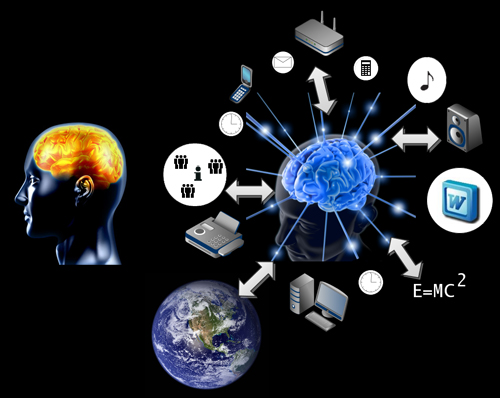
\includegraphics[width=8cm]{images/cognition4.jpg}
		\end{center}
	}
\end{frame}

\begin{frame}
	\frametitle{分布式认知模型}
	\beamertemplatetransparentcovereddynamicmedium
	\begin{itemize}
		\item 在进行分布式认知分析时,通常需要考查:\pause
		\begin{itemize}
			\item 分布式问题的解决方法\\{\tiny 包括协议解决方式}\pause
			\item 语言及非语言行为的任务\\{\tiny 包括说了什么、眼神和眨眼等暗示什么、什么是没有说出来的}\pause
			\item 使用的各种协调机制\\{\tiny 如规则、规程}\pause
			\item 协作活动在进行过程中将用到的各种通信路径\pause
			\item 如何共享和访问信息
		\end{itemize}
	\end{itemize}
\end{frame}

\section{小结}
\begin{frame}
	\frametitle{小结}
	\begin{itemize}
		\item 了解人的感知模型
		\item 掌握认知过程与交互设计原则
		\item 掌握概念模型及对概念模型的认知
		\item 了解分布式认知
	\end{itemize}
\end{frame}
 
\begin{frame}
	\frametitle{参考文献}
	\bibliographystyle{plain}
	\bibliography{hci}
\end{frame}

\end{document}